\documentclass[12pt]{article}
\usepackage[utf8]{inputenc}
\usepackage{booktabs}
\usepackage{geometry}
\usepackage{graphicx}
\geometry{a4paper, margin=1in}
\title{Results of the Fisher Combined Test}
\author{Sara Fraija}
\date{\today}
\begin{document}
\maketitle
\section{Resultados}

\begin{table}[h!]
\centering
\resizebox{\textwidth}{!}{%
\begin{tabular}{l c c c c c c}
\toprule
\textbf{GRB} & \textbf{Transit} & \textbf{Significance} & \textbf{Significance Corregida} & \textbf{p-value} & \textbf{Corrected p-value} & \textbf{PDF} \\ \midrule
GRB170708046 & 1__plus_20 & 0.61 & -0.21 & 7.291e-01 & 5.843e-01 & 6.688e-01 \\
GRB170816599 & 1__plus_20 & 2.13 & 1.69 & 9.834e-01 & 4.540e-02 & 9.587e-01 \\
GRB170222209 & 1__plus_20 & 0.36 & -1.73 & 6.406e-01 & 9.579e-01 & 6.261e-01 \\
GRB170403583 & 1__plus_20 & 0.41 & -1.26 & 6.591e-01 & 8.967e-01 & 6.332e-01 \\
GRB170826369 & 1__plus_20 & 0.56 & -1.53 & 7.123e-01 & 9.369e-01 & 6.590e-01 \\
GRB190515190 & 1__plus_20 & 1.38 & -0.13 & 9.162e-01 & 5.506e-01 & 8.461e-01 \\
GRB150101270 & 1__plus_20 & 2.04 & 2.04 & 9.793e-01 & 2.068e-02 & 9.502e-01 \\
GRB150101641 & 1__plus_20 & 1.52 & 1.52 & 9.357e-01 & 6.426e-02 & 8.743e-01 \\
GRB150110923 & 1__plus_20 & 0.17 & 0.17 & 5.675e-01 & 4.325e-01 & 6.068e-01 \\
GRB150120123 & 1__plus_20 & 0.99 & 0.99 & 8.389e-01 & 1.611e-01 & 7.556e-01 \\
GRB150922234 & 1__plus_20 & 2.01 & 2.01 & 9.778e-01 & 2.222e-02 & 9.471e-01 \\
GRB151228129 & 1__plus_20 & 0.00 & -0.00 & 5.000e-01 & 5.000e-01 & 6.011e-01 \\
GRB151229285 & 1__plus_20 & 0.90 & 0.90 & 8.159e-01 & 1.841e-01 & 7.339e-01 \\
GRB160612842 & 1__plus_20 & 2.41 & 2.41 & 9.920e-01 & 7.976e-03 & 9.781e-01 \\
GRB160624477 & 1__plus_20 & 0.17 & 0.17 & 5.675e-01 & 4.325e-01 & 6.068e-01 \\
GRB160726065 & 1__plus_20 & 1.99 & 1.99 & 9.767e-01 & 2.330e-02 & 9.449e-01 \\
GRB170318644 & 1__plus_20 & 2.86 & 2.86 & 9.979e-01 & 2.118e-03 & 9.933e-01 \\
GRB170325331 & 1__plus_20 & 0.00 & -0.00 & 5.000e-01 & 5.000e-01 & 6.011e-01 \\
GRB170803729 & 1__plus_20 & 1.97 & 1.97 & 9.756e-01 & 2.442e-02 & 9.427e-01 \\
GRB170817529 & 1__plus_20 & 1.86 & 1.86 & 9.686e-01 & 3.144e-02 & 9.293e-01 \\
GRB180204109 & 1__plus_20 & 0.76 & 0.76 & 7.764e-01 & 2.236e-01 & 7.011e-01 \\
GRB180418281 & 1__plus_20 & 1.18 & 1.18 & 8.810e-01 & 1.190e-01 & 8.011e-01 \\
GRB180715755 & 1__plus_20 & 2.88 & 2.88 & 9.980e-01 & 1.988e-03 & 9.937e-01 \\
GRB180718082 & 1__plus_20 & 2.56 & 2.56 & 9.948e-01 & 5.234e-03 & 9.849e-01 \\
GRB180805543 & 1__plus_20 & 0.00 & -0.00 & 5.000e-01 & 5.000e-01 & 6.011e-01 \\
GRB181125371 & 1__plus_20 & 1.84 & 1.84 & 9.671e-01 & 3.288e-02 & 9.266e-01 \\
GRB190427190 & 1__plus_20 & 0.00 & -0.00 & 5.000e-01 & 5.000e-01 & 6.011e-01 \\
GRB201008443 & 1__plus_20 & 2.05 & 2.05 & 9.798e-01 & 2.018e-02 & 9.512e-01 \\
GRB201214672 & 1__plus_20 & 1.20 & 1.20 & 8.849e-01 & 1.151e-01 & 8.058e-01 \\
GRB210323918 & 1__plus_20 & 2.10 & 2.10 & 9.821e-01 & 1.786e-02 & 9.560e-01 \\
GRB211024065 & 1__plus_20 & 0.00 & -0.00 & 5.000e-01 & 5.000e-01 & 6.011e-01 \\
GRB220412713 & 1__plus_20 & 0.94 & 0.94 & 8.264e-01 & 1.736e-01 & 7.435e-01 \\
GRB220418720 & 1__plus_20 & 0.35 & 0.35 & 6.368e-01 & 3.632e-01 & 6.248e-01 \\
GRB220511571 & 1__plus_20 & 1.47 & 1.47 & 9.292e-01 & 7.078e-02 & 8.646e-01 \\
GRB220617772 & 1__plus_20 & 1.60 & 1.60 & 9.452e-01 & 5.480e-02 & 8.891e-01 \\
GRB221120895 & 1__plus_20 & 0.51 & 0.51 & 6.950e-01 & 3.050e-01 & 6.497e-01 \\
GRB230228244 & 1__plus_20 & 0.00 & -0.00 & 5.000e-01 & 5.000e-01 & 6.011e-01 \\
GRB230512269 & 1__plus_20 & 0.00 & -0.00 & 5.000e-01 & 5.000e-01 & 6.011e-01 \\
GRB230812790 & 1__plus_20 & 0.88 & 0.88 & 8.106e-01 & 1.894e-01 & 7.291e-01 \\
GRB150819440 & 2__plus_20 & 0.00 & -1.05 & 5.000e-01 & 8.542e-01 & 6.011e-01 \\
GRB170708046 & 2__plus_20 & 0.00 & -1.05 & 5.000e-01 & 8.542e-01 & 6.011e-01 \\
GRB170816599 & 2__plus_20 & 1.58 & 1.03 & 9.429e-01 & 1.506e-01 & 8.855e-01 \\
GRB170206453 & 2__plus_20 & 0.59 & -1.45 & 7.224e-01 & 9.265e-01 & 6.648e-01 \\
GRB170222209 & 2__plus_20 & 1.50 & 0.28 & 9.332e-01 & 3.884e-01 & 8.705e-01 \\
GRB170403583 & 2__plus_20 & 1.46 & 0.43 & 9.279e-01 & 3.348e-01 & 8.626e-01 \\
GRB170826369 & 2__plus_20 & 0.00 & -2.69 & 5.000e-01 & 9.965e-01 & 6.011e-01 \\
GRB190515190 & 2__plus_20 & 1.30 & -0.27 & 9.032e-01 & 6.057e-01 & 8.286e-01 \\
GRB141205337 & 2__plus_20 & 0.00 & -0.00 & 5.000e-01 & 5.000e-01 & 6.011e-01 \\
GRB150101270 & 2__plus_20 & 1.19 & 1.19 & 8.830e-01 & 1.170e-01 & 8.035e-01 \\
GRB150101641 & 2__plus_20 & 0.44 & 0.44 & 6.700e-01 & 3.300e-01 & 6.379e-01 \\
GRB150922234 & 2__plus_20 & 0.12 & 0.12 & 5.478e-01 & 4.522e-01 & 6.039e-01 \\
GRB151229285 & 2__plus_20 & 2.79 & 2.79 & 9.974e-01 & 2.635e-03 & 9.919e-01 \\
GRB160612842 & 2__plus_20 & 0.92 & 0.92 & 8.212e-01 & 1.788e-01 & 7.387e-01 \\
GRB160624477 & 2__plus_20 & 0.25 & 0.25 & 5.987e-01 & 4.013e-01 & 6.133e-01 \\
GRB160726065 & 2__plus_20 & 0.87 & 0.87 & 8.078e-01 & 1.922e-01 & 7.268e-01 \\
GRB170318644 & 2__plus_20 & 0.40 & 0.40 & 6.554e-01 & 3.446e-01 & 6.317e-01 \\
GRB170325331 & 2__plus_20 & 2.21 & 2.21 & 9.864e-01 & 1.355e-02 & 9.653e-01 \\
GRB170803729 & 2__plus_20 & 1.33 & 1.33 & 9.082e-01 & 9.176e-02 & 8.353e-01 \\
GRB170817529 & 2__plus_20 & 1.91 & 1.91 & 9.719e-01 & 2.807e-02 & 9.356e-01 \\
GRB171007498 & 2__plus_20 & 0.00 & -0.00 & 5.000e-01 & 5.000e-01 & 6.011e-01 \\
GRB180204109 & 2__plus_20 & 0.00 & -0.00 & 5.000e-01 & 5.000e-01 & 6.011e-01 \\
GRB180402406 & 2__plus_20 & 1.63 & 1.63 & 9.484e-01 & 5.155e-02 & 8.943e-01 \\
GRB180418281 & 2__plus_20 & 0.97 & 0.97 & 8.340e-01 & 1.660e-01 & 7.508e-01 \\
GRB180715755 & 2__plus_20 & 0.00 & -0.00 & 5.000e-01 & 5.000e-01 & 6.011e-01 \\
GRB180718082 & 2__plus_20 & 0.86 & 0.86 & 8.051e-01 & 1.949e-01 & 7.244e-01 \\
GRB180805543 & 2__plus_20 & 0.27 & 0.27 & 6.064e-01 & 3.936e-01 & 6.153e-01 \\
GRB181125371 & 2__plus_20 & 0.00 & -0.00 & 5.000e-01 & 5.000e-01 & 6.011e-01 \\
GRB190427190 & 2__plus_20 & 1.16 & 1.16 & 8.770e-01 & 1.230e-01 & 7.964e-01 \\
GRB200415367 & 2__plus_20 & 0.00 & -0.00 & 5.000e-01 & 5.000e-01 & 6.011e-01 \\
GRB201008443 & 2__plus_20 & 0.00 & -0.00 & 5.000e-01 & 5.000e-01 & 6.011e-01 \\
GRB201214672 & 2__plus_20 & 1.03 & 1.03 & 8.485e-01 & 1.515e-01 & 7.653e-01 \\
GRB210323918 & 2__plus_20 & 0.00 & -0.00 & 5.000e-01 & 5.000e-01 & 6.011e-01 \\
GRB210618072 & 2__plus_20 & 0.00 & -0.00 & 5.000e-01 & 5.000e-01 & 6.011e-01 \\
GRB220412713 & 2__plus_20 & 1.39 & 1.39 & 9.177e-01 & 8.226e-02 & 8.482e-01 \\
GRB220418720 & 2__plus_20 & 0.93 & 0.93 & 8.238e-01 & 1.762e-01 & 7.411e-01 \\
GRB220511571 & 2__plus_20 & 1.53 & 1.53 & 9.370e-01 & 6.301e-02 & 8.762e-01 \\
GRB220617772 & 2__plus_20 & 1.39 & 1.39 & 9.177e-01 & 8.226e-02 & 8.482e-01 \\
GRB221120895 & 2__plus_20 & 0.00 & -0.00 & 5.000e-01 & 5.000e-01 & 6.011e-01 \\
GRB230228244 & 2__plus_20 & 3.08 & 3.08 & 9.990e-01 & 1.035e-03 & 9.965e-01 \\
GRB230512269 & 2__plus_20 & 0.40 & 0.40 & 6.554e-01 & 3.446e-01 & 6.317e-01 \\
GRB230812790 & 2__plus_20 & 3.18 & 3.18 & 9.993e-01 & 7.364e-04 & 9.975e-01 \\
\bottomrule
\end{tabular}%
}
\caption{Lista de GRBs with sus Transits, Significances, Significances Corregidas, p-values, p-values Corregidos y valores PDF.}
\end{table}

\begin{figure}[h!]
\centering
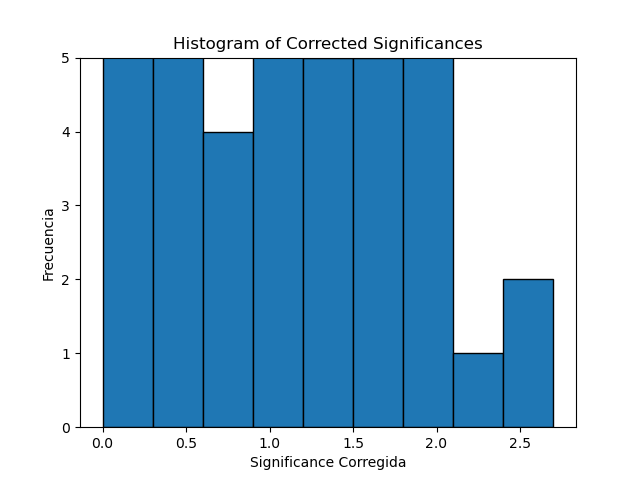
\includegraphics[width=0.6\textwidth]{corrected_significance_hist.png}
\caption{Histogram of Corrected Significances.}
\end{figure}

\section*{Conclusion}
The Fisher combined test integrates individual p-values to evaluate a global hypothesis.
The resulting test statistic was $X^2 = 319.865$ with 162 degrees of freedom.
For a significance level of 0.05, the critical value is 192.700.
Since $X^2$ is greater than the critical value, we rechazamos the null hypothesis of independence.
Normal approximation: p-value = 2.430e-12, significance ≈ 6.91 sigma.

\end{document}